\documentclass[11pt,fleqn]{article}

\setlength {\topmargin} {-.15in}
\setlength {\textheight} {8.6in}

\usepackage{amsmath}
\usepackage{amssymb}
\usepackage{color}
\usepackage{tikz}
\usetikzlibrary{automata,positioning,arrows}
\usepackage{diagbox}



\newcommand{\be}{\begin{enumerate}}
\newcommand{\ee}{\end{enumerate}}

\begin{document}

\textbf{Exercise 4.2.19:} Topological sort and BFS. Explain why the following algorithm does not necessarily
produce a topological order: Run BFS, and label the vertices by increasing distance
to their respective source.\\

\textbf{Solution:}\\
No, counterexample below. Recall BFS is level order traversal due to the use of a Queue.

\begin{center}
	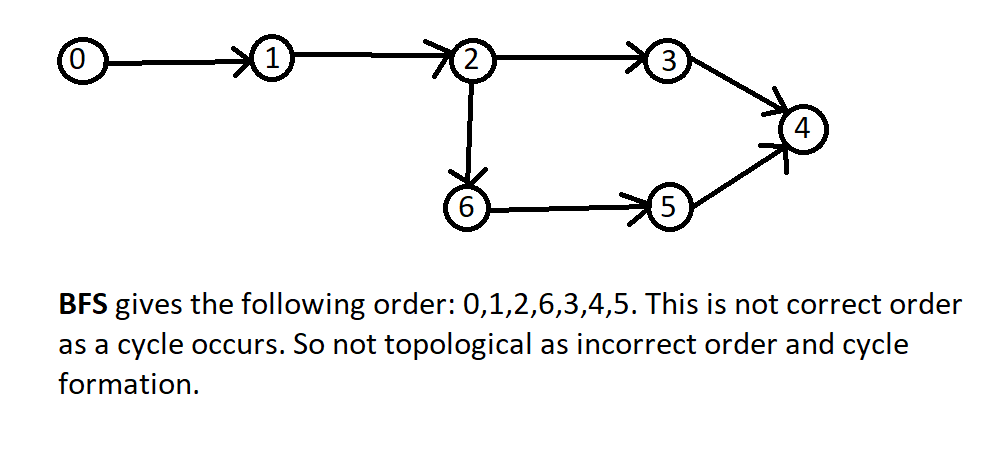
\includegraphics[scale=.6]{4.2.19.png}
\end{center}


	


\end{document}
